\documentclass{slide}
\usepackage{tikz}

\usetikzlibrary{arrows}


\title{Distributed Computing I}
\subtitle{CSSE6400}
\author{Brae Webb}
\date{\week{5}}

\titlegraphic {
    \tweet%
    {images/mathiasverraes}%
    {Mathias Verras}%
    {mathiasverraes}%
    {There are only two hard problems in distributed systems:  2. Exactly-once delivery 1. Guaranteed order of messages 2. Exactly-once delivery}%
    {https://twitter.com/mathiasverraes/status/632260618599403520}%
}

\begin{document}

\maketitle

\point[Fallacy \#1]{The network is reliable}

\image{diagrams/working}

\image{diagrams/drop1}

\image{diagrams/dropRecover}

\image{diagrams/dropRecoverDos}

\image{diagrams/drop2}

\image{diagrams/drop2Recovery}

\image{diagrams/drop2Fix}

\point[Fallacy \#2]{Latency is zero}

\point[Fallacy \#3]{Bandwidth is infinite}

\point[Fallacy \#4]{The network is secure}

\point[Fallacy \#5]{The topology never changes}

\point[Fallacy \#6]{There is only one administrator}

\point[Fallacy \#7]{Transport cost is zero}

\point[Fallacy \#8]{The network is homogeneous}


\point[Focus]{Reliability}

\question{What makes software \highlight{unreliable}?}

\point[`Working' software]{Satisfies the functional requirements}

\definition{Reliable Software}{Continues to work correctly, even when things go wrong.}

\definition{Fault}{Something goes wrong.}

\quote[Howard and LeBlanc]{Death, taxes, and computer system failure are all inevitable to some degree.\\\highlight{Plan for the event.}}

\point[Reliable software is]{Fault tolerant}
    
\point[Problem]{Individual computers fail \highlight{all the time}}

\point[Solution]{Spread the risk of faults over \highlight{multiple computers}}

\point[Spreading Risk]{
    \large
    If you have software that works with \highlight{just one} computer,
    spreading the software over \highlight{two} computers \highlight{halves} the risk that your software will fail.
    \\[2em]
    \only<2->{Adding \highlight{10} computers reduces the cuts the risk by \highlight{10}.}
    \extra[3-]{Of course, there are other reasons you might want run software on multiple computers.}
}

\definition{Distributed Computing}{Multiple software components that are on multiple computers, but run as a single system}

\point[The Problem]{
    \begin{center}
    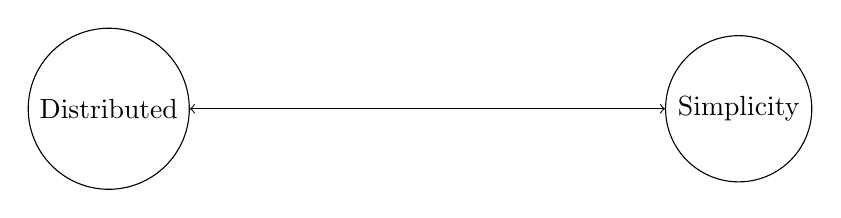
\begin{tikzpicture}
        \node[circle,draw, minimum size=1cm] (A) at  (0,0) {Distributed};
        \node[circle,draw, minimum size=1cm] (B) at  (8,0)  {Simplicity};
        \draw[<->] (A) -- (B);
    \end{tikzpicture}
    \end{center}
}

\point{A lot of modern software development focuses on dealing with the \highlight{complexity} of distributed systems.}

\question{What makes distributed computing complex?}

\point{
    \begin{itemize}
        \item Faults
        \item Asynchronous communication
        \item Monitoring
        \item And much more\dots
    \end{itemize}
}


% \references{articles,books}

\end{document}